% Fig. 7 -- Detection-event pipeline: admission checks, then scoring and decision (full width, 7.16 in).
% Compile with pdfLaTeX (Overleaf default). Output: fig07_event_pipeline.pdf
\documentclass[border=3pt]{standalone}
\usepackage[T1]{fontenc}
\usepackage{newtxtext,newtxmath}
\usepackage{tikz}
\usetikzlibrary{arrows.meta,positioning,calc}

\definecolor{acc}{RGB}{31,78,121}
\colorlet{accfill}{acc!10}
\colorlet{gfill}{black!7}

\tikzset{
  >={Stealth[length=3pt,width=2.6pt]},
  every node/.style={font=\footnotesize},
  adm/.style={draw=black,line width=0.5pt,fill=white,align=center,inner sep=2pt,
              minimum width=74pt,minimum height=30pt},
  stp/.style={draw=black,line width=0.5pt,fill=white,align=center,inner sep=2pt,
              minimum width=66pt,minimum height=30pt},
  accn/.style={draw=acc,fill=accfill,line width=0.7pt},
  src/.style={fill=gfill},
  flow/.style={->,line width=0.5pt},
  stagelabel/.style={inner sep=1pt,font=\footnotesize\bfseries},
}

\begin{document}
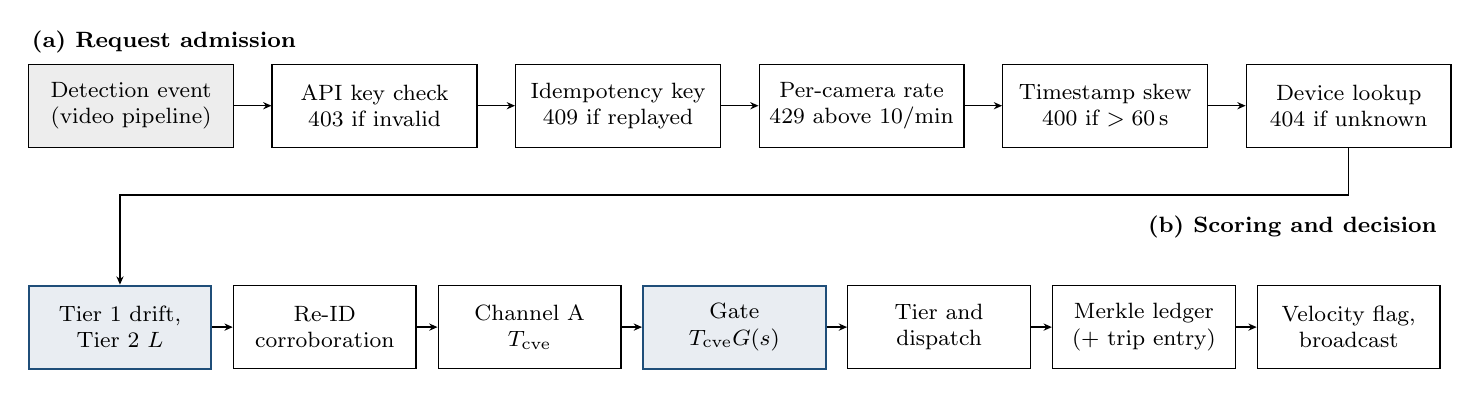
\begin{tikzpicture}[x=1pt,y=1pt]
  % ---------- (a) admission
  \node[stagelabel,anchor=south west] at (0,18) {(a) Request admission};
  \node[adm,src] (n1) at (37,0)  {Detection event\\(video pipeline)};
  \node[adm]     (n2) at (125,0) {API key check\\403 if invalid};
  \node[adm]     (n3) at (213,0) {Idempotency key\\409 if replayed};
  \node[adm]     (n4) at (301,0) {Per-camera rate\\429 above 10/min};
  \node[adm]     (n5) at (389,0) {Timestamp skew\\400 if $>60$\,s};
  \node[adm]     (n6) at (477,0) {Device lookup\\404 if unknown};
  \draw[flow] (n1.east) -- (n2.west);
  \draw[flow] (n2.east) -- (n3.west);
  \draw[flow] (n3.east) -- (n4.west);
  \draw[flow] (n4.east) -- (n5.west);
  \draw[flow] (n5.east) -- (n6.west);

  % ---------- (b) scoring and decision
  \node[stagelabel,anchor=south east] at (510,-49) {(b) Scoring and decision};
  \node[stp,accn] (m1) at (33,-80)  {Tier 1 drift,\\Tier 2 $L$};
  \node[stp]      (m2) at (107,-80) {Re-ID\\corroboration};
  \node[stp]      (m3) at (181,-80) {Channel A\\$T_{\mathrm{cve}}$};
  \node[stp,accn] (m4) at (255,-80) {Gate\\$T_{\mathrm{cve}}G(s)$};
  \node[stp]      (m5) at (329,-80) {Tier and\\dispatch};
  \node[stp]      (m6) at (403,-80) {Merkle ledger\\(+ trip entry)};
  \node[stp]      (m7) at (477,-80) {Velocity flag,\\broadcast};
  \draw[flow] (m1.east) -- (m2.west);
  \draw[flow] (m2.east) -- (m3.west);
  \draw[flow] (m3.east) -- (m4.west);
  \draw[flow] (m4.east) -- (m5.west);
  \draw[flow] (m5.east) -- (m6.west);
  \draw[flow] (m6.east) -- (m7.west);

  % ---------- hand-over from (a) to (b)
  \draw[flow] (n6.south) -- ++(0,-17) -| (m1.north);
\end{tikzpicture}
\end{document}
